%
% File acl2017.tex
%
%% Based on the style files for ACL-2015, with some improvements
%%  taken from the NAACL-2016 style
%% Based on the style files for ACL-2014, which were, in turn,
%% based on ACL-2013, ACL-2012, ACL-2011, ACL-2010, ACL-IJCNLP-2009,
%% EACL-2009, IJCNLP-2008...
%% Based on the style files for EACL 2006 by 
%%e.agirre@ehu.es or Sergi.Balari@uab.es
%% and that of ACL 08 by Joakim Nivre and Noah Smith

\documentclass[11pt,a4paper]{article}
\usepackage[hyperref]{acl2017}
\usepackage{times}
\usepackage{latexsym}


%for the table
\usepackage{booktabs}

%for [H]
\usepackage{float}
\usepackage{graphicx}

\usepackage{url}

\aclfinalcopy % Uncomment this line for the final submission
%\def\aclpaperid{***} %  Enter the acl Paper ID here

%\setlength\titlebox{5cm}
% You can expand the titlebox if you need extra space
% to show all the authors. Please do not make the titlebox
% smaller than 5cm (the original size); we will check this
% in the camera-ready version and ask you to change it back.

\newcommand\BibTeX{B{\sc ib}\TeX}

\title{Evaluation of Neural Networks for Multi-Class Emoji Prediction}

\author{Yun Zhang \\
	 104946985 \\
	% \\
	 \\
	\small{\tt zhangmike@ucla.edu } \\\And
	Peter Kim \\
	204271299 \\
%	 \\
	 \\
	\small{\tt peterkim95@ucla.edu} \\\And
	Haoxiang Zhang \\
	104278461 \\
	% \\
	 \\
	\small{\tt zhanghaoxiang@ucla.edu} \\\And
	 Jonathan Hurwitz \\
	 804258351 \\
%	 \\
	 \\
	\small{\tt jdhurwitz@ucla.edu} \\
}
\date{}

\begin{document}
	\maketitle
	\begin{abstract}
	Emoji prediction has become a popular task in Natural Language Processing. The goal of the task is to predict and select the most possible emoji used in the original tweet from the emoji list given the text information. We performed experiments on different neural network models and hyperparameters to find out the model with the best performance. We explore the simple feed-forward neural network to get an idea of baseline performance before moving on towards the evaluation and design of more complicated models, such as GRU, Bi-GRU, LSTM, and Bi-LSTM. Given the experiment results, we visualize the classifier performance results via confusion matrices, and compare them between different models.
	\end{abstract}
	
	\section{Introduction}
	
	Modern users spend a significant amount of time on social networking services (SNS), such as Twitter and Instagram. Huge amounts of data are generated at rapid speed. Across all popular social networking platforms, Emojis are used in addition to basic text. These provide an additional layer of meaning to the textual data, and can even be considered as pictorial summarizations of the text. Inspired by this idea, we want to create out a robust model to extract useful patterns from the data, explore the underlying relationship between Emojis and text, and predict the most likely Emoji(s) given an associated text.
	\par
	The previous work on this topic hasn’t achieved a good performance on general predictions due to the imbalanced proportion of the dataset. It is obvious that a certain number of emojis is used by people quite often while the frequency of the rest is quite low. The models they derived tend to overfit the training data and give a bad performance on the test dataset if emojis with low frequency appear more than normal.
	\par
	This project was inspired by the emoji prediction project hosted on CodaLab. The data they provided consists of 500k tweets in English and 100k tweets in Spanish. We’ve focused on emoji prediction for English. Tweet dates span the range from October 2015 to February 2017 and are geolocalized to the US and Spain. The dataset was built from tweets that contain one and only one of the twenty most frequent emojis. The label set consists of the twenty most frequent emojis labeled numerically from 0-19.
	
	
	\begin{figure}[H]
		%\hspace*{-1.3cm}
		\centering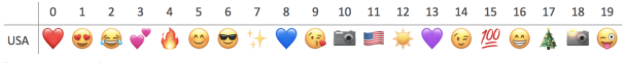
\includegraphics[scale=0.36]{emojis} 
		\caption{\textbf{ Mapping from emojis to numerical values.}}
	\end{figure}
	
	
	The main goal of this competition is to create a classifier to predict the emoji used in the tweet given the text data with maximum macro F1 score. Our approach focused on evaluating several neural network architectures, starting with the simplest single-layer feed-forward model and extending to bidirectional RNN-based models. Our goal is to figure out a robust neural network model to predict the emoji used in tweets under general cases. We test several neural network model structures, various pre-trained word embedding methods, and tune the parameters to get the best performance. Post-validation model analysis is primarily focused on trying to understand model classification tendencies, such as over emphasis of frequent emojis. Confusion matrices are used as a performance visualization. 
	\par
	The learned models and code for developing the architectures can be found in the following github repository: \url{https://github.com/peterkim95/tweet-emoji-predictor}.  The rest of the paper is organized as follows. Methods on the data preprocessing, the selection of pre-trained word data and models are discussed in section 2. Section 3 shows and analyzes the results from the experiments. Section 4 gives conclusions and future work on this task.
	
	\section{Data}
	\subsection{Preprocessing}
	Since the raw tweet data contains a large number of meaningless signs and irregular slang which could negatively impact the performance of the model, we first need to remove noise from the data. We delete whitespace, change all the words to lowercase, remove ‘...’, split compound words into separate ones, eliminate repeating characters (e.g. no wayyyy -> no way), and remove ‘@’ and ‘\#’ signs. We also use a compound word splitter to generate a new phrase given a single hashtag (e.g. \#lovewins -> love wins), as the meaning embedded in hashtags still carry semantic value, and therefore is wasteful to ignore. Then we tokenize those sentences into word lists and build up a vocabulary according to those lists.
	
	\subsection{Word Embedding Methods}
	We tested three methods to create word vectors and generate word embeddings. The first one is to use word vectors generated randomly. The second one is to use GloVe Embeddings trained on Wikipedia corpus. 
	\par
	After applying the standard NLTK tokenizer to split a tweet into a list of words, and applying the preprocessing steps described before, we embed the words using either a randomly initialized or pretrained GloVe word embeddings.
	\par
	The final method involved using the pretrained vectors trained on part of Google News dataset using the Word2vec model. Google’s word2vec model includes word vectors for a vocabulary of 3 million words and phrases, trained on 100 billion words from Google News. Each vector has dimension 300. Word embeddings were done by taking Google’s pretrained news vectors and performing mean aggregation on each tweet to create a tweet vector. The preprocessing step for the MLP model involves pulling all the tweets and tokenizing them. Unlike the preprocessing for later models discussed, the tokenization did not involve removing any words and was simply to split up a tweet’s word sequence into a list of words. A word embedding matrix was created by scanning through each tweet in the dataset, and for each word within the tweet, checking to see if the Google word2vec model had a vector representation for the word. If so, this vector became the representation of the word. If no occurence in the model, a zero-padded vector (of dimension 300) served as the representation. At the end of the sequence, the mean of these vectors was calculated as the corresponding “tweet” vector embedding. This mean aggregation method is essentially a form of text summarization into a single vector. This final embedding was the input for the model. This method was meant to serve as a baseline due to its simplicity. It was only used with the feed-forward neural net model due to time and resource constraints.
	
	\section{Models}
	
	\subsection{Feed Forward Neural Net}
	Since this is a multi-class classification problem, the basic neural net structure is aptly suited. Multi-class classification can be performed by increasing the number of nodes on the output layer to suit the dimension of the class vector. A function such as softmax can compress these values into a probabilistic range such that the sum of outputs for some input instance is 1. The feed-forward neural net, or multi-layer perceptron (MLP) model was meant to serve as a rough baseline for the project.
	\par
	The MLP invariants included a 300-node input layer (one for each dimension) as well as a 20-node output layer, corresponding to a one-to-one mapping for the class assignments. Several experiments were done to test the effects of hidden layer node number as well as number of hidden layers. Due to time constraints, a full cross-validation and hyper parameter tuning exercise was not performed. 
	\par
	One criticism of MLP for sentiment analysis is the simplicity of the model in that it can’t encapsulate long-chain dependencies. There is no notion of a sequence and each data instance exists on its own. Tweets are sufficiently short (due to character limit) such that long-chain dependencies might not necessarily appear, but the more complicated models tested have been historically shown to model such dependencies successfully. 
	
	\begin{figure}[H]
		\hspace*{-1.3cm}
		\centering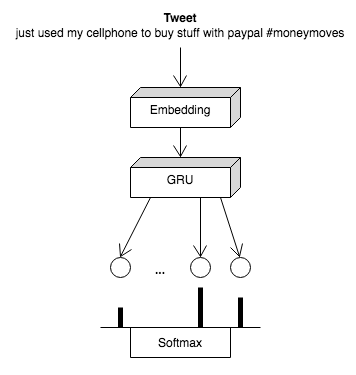
\includegraphics[scale=0.7]{modelgru} 
		\caption{\textbf{ Basic architecture, showing the layers that a tweet goes through prior to classification output.}}
	\end{figure}
	
	
	\subsection{Gated Recurrent Unit (GRU)}
	A recurrent neural network (RNN) is a class of neural network that has connections between units. Unlike the feed-forward neural network, an RNN has memory to capture information that has already been calculated. This feature allows RNN to process arbitrary sequences of inputs. The gated recurrent unit (GRU) is a gating mechanism in RNN. A GRU has a reset gate and an update gate. The reset gate combines the new input with the previous memory, and the update gate decides how much of the previous memory should be kept. The GRU model serves as one of more complicated models that should be more accurate than our baseline MLP model.
	
	\begin{figure}[H]
		%\hspace*{-1.3cm}
		\centering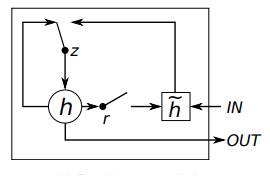
\includegraphics[scale=0.7]{gru} 
		\caption{\textbf{ GRU. Chung, Junyoung, et al. “Empirical evaluation of gated recurrent neural networks on sequence modeling.” (2014).}}
	\end{figure}

	
	
	
	\subsection{Bidirectional Gated Recurrent Unit (Bi-GRU)}
	\label{sect:pdf}
	
	Besides the standard gated recurrent unit (GRU), we also implemented a bidirectional gated recurrent unit (Bi-GRU). Bi-GRU was used to increase the amount of information available to the recurrent neural network. By constructing neurons in both forward and backward directions, the current state of of Bi-GRU can obtain information from past and future states. This is extremely useful when understanding the context of input, especially for longer bodies of texts. However, since tweets are generally no more than 20 words, we expect that this bidirectional model will have a marginal performance gain over the previous GRU model.
	

	
	\subsection{Long Short Term Memory (LSTM)}
	
	Like the GRU, the LSTM has a notion of memory. Its memory cell consists of four main elements: an input gate, a neuron with a path back to itself, a forget gate, and an output gate. The loop back allows the state of a memory cell to remain constant through time. The forget gate modulates the loop back and can allow the cell to “delete” or “forget” its previous state. LSTMs do not suffer from the vanishing or exploding gradient problem when long sequences are processed. It is an effective model for data that exhibits long-chain dependencies. We expect that this model will perform similarly to the GRU model, but will take longer to train as LSTMs are more computationally expensive than GRUs.  
	
	 
	
	\begin{figure}[H]
	%	\hspace*{-1.3cm}
		\centering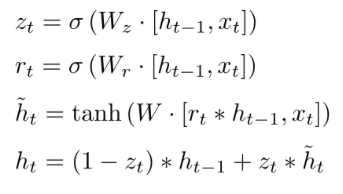
\includegraphics[scale=0.5]{lstm_functions} 
		\caption{\textbf{ LSTM functions.}}
	\end{figure}
	\subsection{Bidirectional Long Short Term Memory (Bi-LSTM)}
	LSTMs only preserve past information because inputs that have been seen are from the past. A bidirectional model allows the inputs to run in the positive and negative direction, at the same time. This is essentially like getting a past view and future view of information. With a bidirectional LSTM, at any point in time you can preserve information from both past and future information.
	
	
\section{Results}

For evaluation, we used accuracy as well as the F1 score, which is a harmonic mean of precision and recall. The task is evaluated based on Macro F-score, as the fundamental idea of this task is to encourage systems to perform well overall, which would inherently mean a better sensitivity to the use of emojis in general rather than overfitting a model to do well in the  three or four most common emojis of the test data. Macro F-score can be defined as simply the average of the individual label-wise F-scores.


\par
To generate a large training dataset, we used Tweepy to crawl about 480,000 tweets with exactly one emoji among the top 20 emojis in English tweets. After training our models on this body of tweets, we tested on the trial dataset provided by the competition hosts, which contains 50,000 tweets. We build a vocabulary based on the training dataset and use <UNK> for unknown words at test time. We choose word embedding size d = 300, and use the 300 dimensional pre-trained GloVe word embeddings from Stanford. The dimension of the hidden layer is 200 and the output size is 20 according to 20 labels we need to predict from. Optimization is carried out using Adam. In addition, we use a mini-batch size of 32, set the learning rate at 1e-3 and train the model for 500 epochs.


\subsection{Comparison of Model Accuracy and F1}
The table below shows a comparison of the F1-scores and dev accuracies for each of the five models. The feed-forward neural net, or multi-layer perceptron (MLP) performed the best with a dev accuracy of 73.9\%, and an F1-score of 58.2. The fact that the F1-score is much lower than accuracy might indicate that this model is predicting the most common emojis rather than encapsulating information inherent in the text that lends itself to accurate predictions.
	\begin{table}[htp]
	%	\hspace*{-4cm}
		\centering
		\caption{F1-Score and Accuracy for Dev Set}
		\label{my-label}
		\begin{tabular}{@{}lll@{}}
			\toprule
			Model       & F1-Score & Dev Accuracy \\ \midrule
			FF NN (MLP) & 58.2     & 73.9         \\
			GRU         & 45.7     & 50.3         \\
			Bi-GRU      & 43.3        & 48.7            \\
			LSTM        & 45.1     & 50.2         \\
			Bi-LSTM     & 43.1       & 47.9            \\ \bottomrule
		\end{tabular}
	\end{table}
%	\section*{Acknowledgments}

\subsection{MLP Tuning}
The table below shows various parameter selections and corresponding F1-Score as well as dev accuracy for the MLP. A maximum of two layers were used in tests. HLx size refers to the number of nodes in hidden layer of depth x. The first experiment involved a single hidden layer with 100 nodes; this is the default for sklearn’s MLPClassifier model and was used as a baseline. F1-Score was poor but accuracy was reasonably high and greater than a random class selection. The second experiment involved adding a hidden layer with the name number of nodes. This increased the F1-Score and increased the accuracy marginally.

\begin{table}[htp]
%	\hspace{-4cm}
%\hskip-4.0cm
	\centering
	\caption{MLP Model Parameters and Results}
	\label{my-label}
	%\hspace{-1.5cm}
	\begin{tabular}{@{}lllll@{}}
		\toprule
		Model       & HL1 size & HL2 size & F1-Score & Dev Accuracy \\ \midrule
		MLP1 		& 100     & 0  &     37.1 & 60.1  \\
		MLP2        & 100     & 100    &   46.5 & 71.3 \\
		MLP3     	& 140     & 0   &     45.8 & 70.7    \\
		MLP4        & 140     & 140    &   58.2 & 73.9  \\ \bottomrule

	\end{tabular}
\end{table} 
Since tweets are 140 characters long, 140 was chosen as a reasonable guess for the number of nodes in the hidden layer. The same experiments were run, first with a single hidden layer of size 140 and then with two hidden layers of the same size. The single hidden layer of size 140 (MLP3) performed marginally worse than the two-layer NN with 100 nodes per layer (MLP2). This indicates that deeper networks are better suited to this task. The final model with two hidden layers of size 140 (MLP4) performed the best in every category. F1-Score improved dramatically but accuracy increased only marginally.

\subsection{Discussion}
	The FF NN model performed significantly better than our RNN models. We believe this is because the sequences in tweets are too short, and therefore does not capture any useful sequential information. Also, emojis are usually dependent on only a single word in a tweet and not the whole semantic meaning of the tweet. Therefore, the sequence information captured by RNNs in general could be ultimately unhelpful for predicting the emoji used.
	\par
	The figures below show the confusion matrices for the feed-forward neural net, GRU, and Bi-GRU respectively. The density along the diagonal of the matrix indicates that most predictions were aligned to the correct class. However, predictions were still biased toward the most common classes.
	\begin{figure}[H]
		\hspace*{-1cm}
		\centering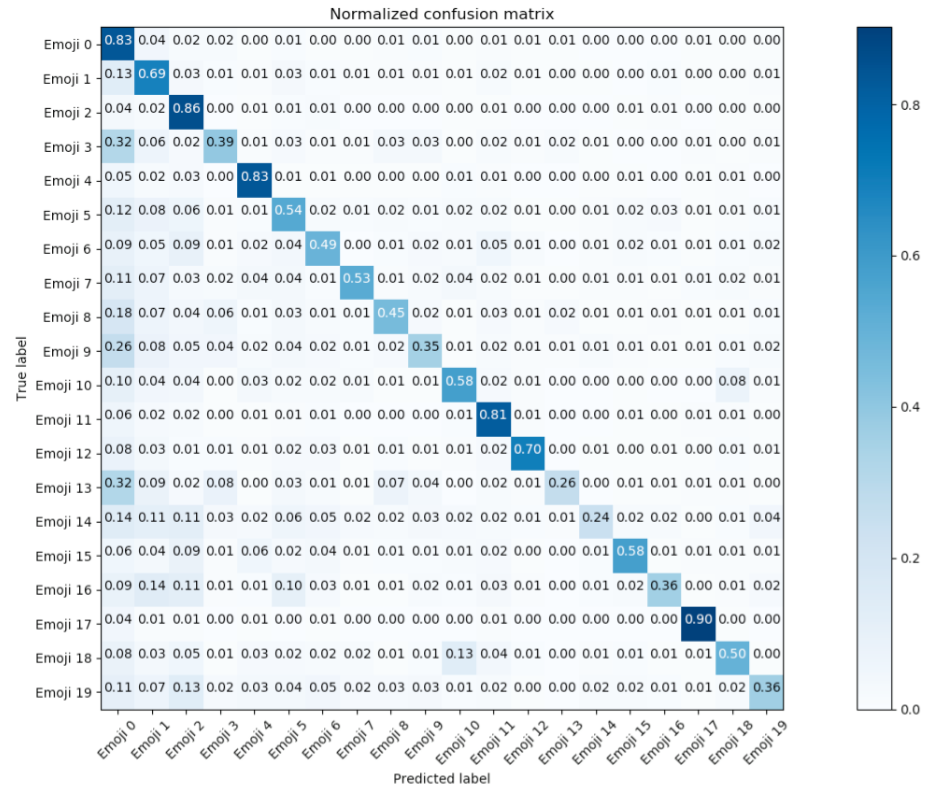
\includegraphics[scale=0.27]{ffnn_confusion} 
		\caption{\textbf{Feed-forward neural network confusion matrix.}}
	\end{figure}
	Apart from the overfitting problem, we noticed an interesting entry in the GRU confusion matrix. The prediction accuracy of emoji 12 in ground truth is quite low but biased to emoji 6. The emoji mapping in Figure 1. shows that emoji 12 is a shining sun whereas emoji 6 is a face with sunglasses on. While there is classification error because these two are different and not being classified correctly, it's interesting to note that our model has captured an implicit similarity between two emojis. These two emojis are similar in semantic meaning but the GRU gets confused. The FF NN achieves good performance in this case so we infer that one or two keywords, rather than the semantic relationship in short sentence sequences, determines the usage of emojis. 
	

	\begin{figure}[H]
		%\hspace*{-1.3cm}
		\centering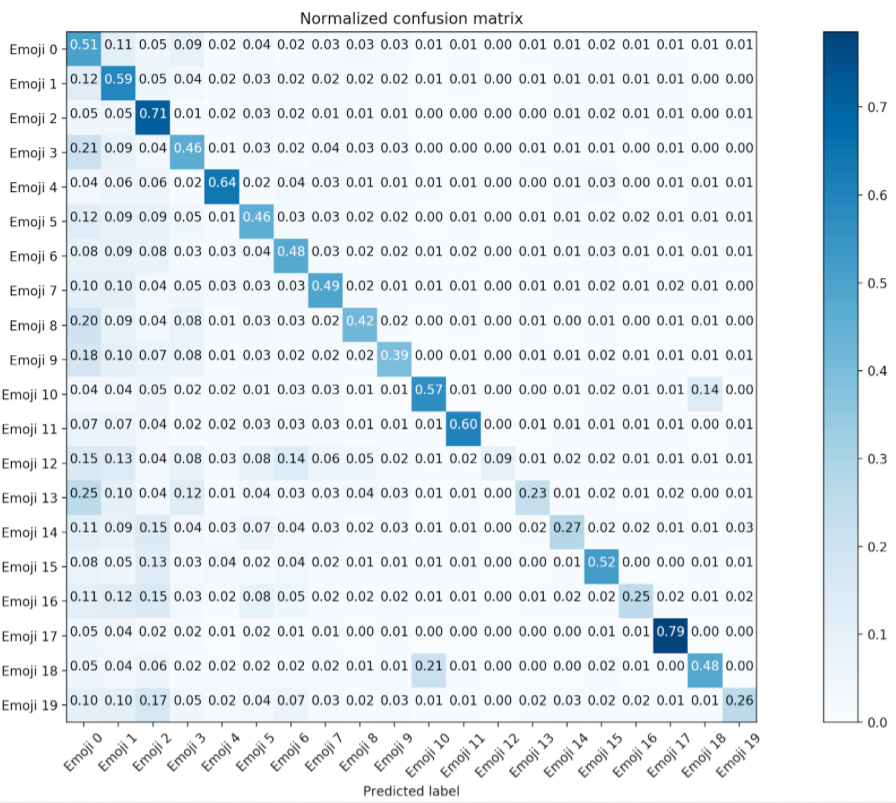
\includegraphics[scale=0.25]{gru_confusion} 
		\caption{\textbf{GRU confusion matrix.}}
	\end{figure}
		The Bi-GRU confusion matrix looks very similar to that of the GRU. It made the same classification error between emojis 6 and 12.
	
	\begin{figure}[H]
		%\hspace*{-1.3cm}
		\centering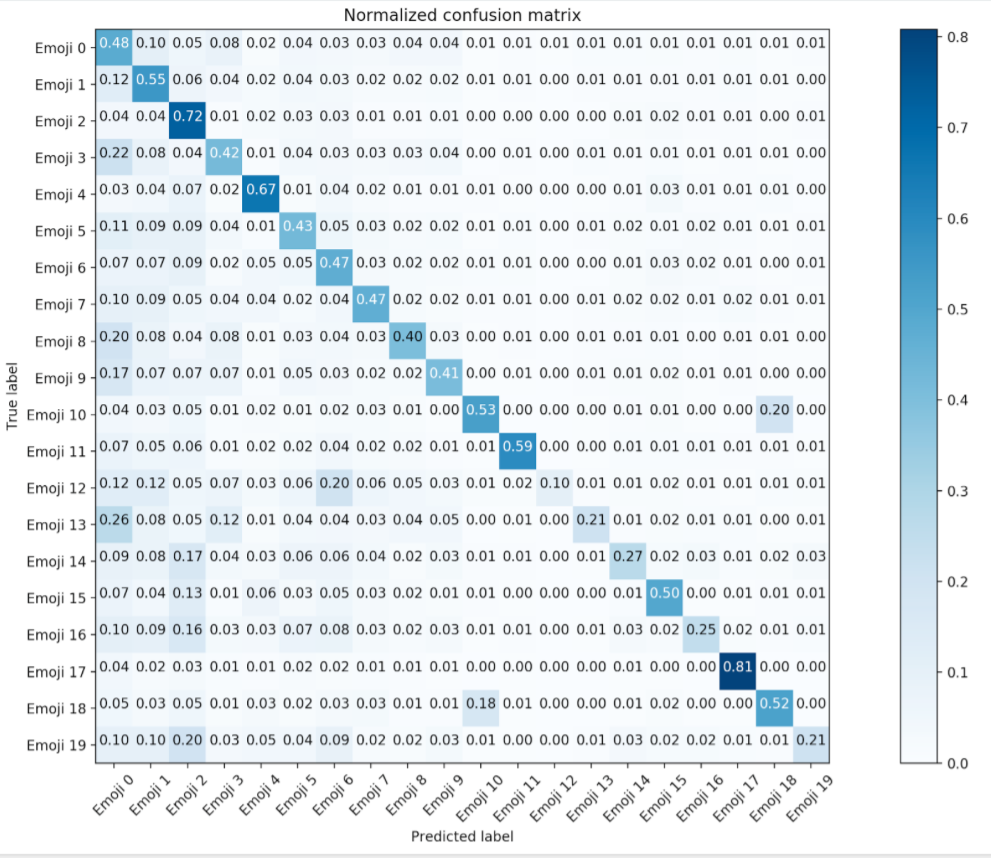
\includegraphics[scale=0.23]{bgru_confusion} 
		\caption{\textbf{Bi-GRU confusion matrix.}}
	\end{figure}

	The hypothesis that an emoji is dependent on the word and not the sequence of words is further strengthened by the following observation: there was a severe performance drop (~20\%) when we use a low dimensional word embedding (d = 50). Here, we realize that using a lower dimensional embedding loses information of each word and semantic meaning between words. This meaning, we hypothesize, is the most critical aspect to correctly predicting an emoji.
	\par
	As hypothesized, both the GRU and LSTM models performed very similarly, and the LSTM model took ~10 minutes more for training a single epoch. 
\section{Future Work}
It appears that word embedding method and dimension have a huge effect on model performance. We’d like to explore other methods of word embedding rather than the previously discussed mean aggregation method and GloVe method. Due to constrained resources and time, we did not have the chance to do a perfect comparison between all models and all embedding methods. Future work would involve testing the mean aggregation (with Google pre-trained vectors) method on the more complicated models to get a more normalized basis of comparison.
\par
As previously mentioned, it appears that emojis depend only on a subset of words in the tweet rather than a long chain dependency. Therefore, it makes sense to focus in on a select few words in a tweet, since these would be the best indicator of output emoji. In this situation, adding an attention RNN decoder to generate the prediction might be a good solution and improves the performance a lot. 

\section{Conclusion}
Tasked with predicting an emoji given a tweet, we have examined several different neural network models ranging from simple feed-forward neural nets to more complicated RNN-based models. The one that performed best was the simplest model: the FF NN model. It achieved state-of-the-art results as it sits at second place on the official CodaLab leaderboards. Overall, we think the RNN models are still valuable models that helped us demonstrate our understanding of common NLP techniques in deep learning.

	

% include your own bib file like this:
%\bibliographystyle{acl}
%\bibliography{acl2017}
\nocite{*}
\bibliography{fr_bib}
\bibliographystyle{acl_natbib}



\appendix


	
\end{document}
